\section{Aktoren}

\subsection{Motoren}
Als einzige steuerbare Aktoren dienen uns DC Motoren von Faulhaber mit einem integrierten Reduktionsgetriebe. Es werden 2 pro Rad zum Einsatz kommen um ausreichend Drehmoment erzielen zu können.

\begin{figure}[H]
    \begin{center}
    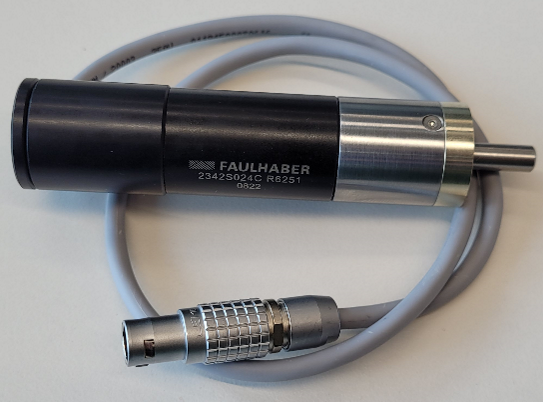
\includegraphics[width=6.3cm]{Aktoren_Motor.png}
    \end{center}
    \caption{Motor}
\end{figure}

\subsection{Peltier Element}
Das Peltier-Element in der Kühlbox erzeugt eine Temperaturdifferenz, sobald man eine Spannung daran anlegt. Mit 2 Lüftern und 2 Kühlelementen, welche in der gekauften Kühlbox bereits vorhanden sind, ist es möglich sowohl zu heizen als auch zu kühlen. \\
\\
Da die Endtemperatur von der Aussentemperatur abhängt, lässt sich hier lediglich eine Temperaturdifferenz sinnvoll definieren, welches ich auf 10-15 Grad festlegen lässt.
\begin{figure}[H]
    \begin{center}
    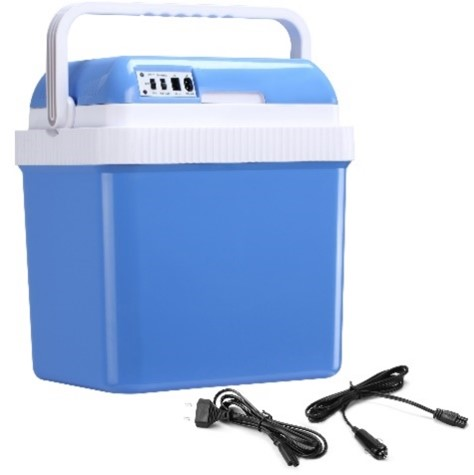
\includegraphics[width=5.5cm]{Aktoren_Peltier Element.jpg}
    \end{center}
    \caption{Kühlbox}
\end{figure}